%============================================%
% Official template for AIDAinnova documents
% to be used for publications using another
% style file than the AIDAinnova one
% For example journal papers, proceedings, etc. 
%
% Updated: 16.05.2022
% Rickard Stroem (lars.rickard.stroem@cern.ch)
%
%============================================%

\documentclass[11pt,a4paper]{scrartcl}

% Defines default style and includes several useful packages
\usepackage{AIDAinnova}

% Useful macros for writing documents
\usepackage{AIDAinnova_definitions}

% Add your packages here
%\usepackage{MyPackage}

%============================================%
% Set up the title page
%============================================%

% Set the title of the note
\title{AIDAinnova Template}

% LICENCE
% Note that all documents (except for drafts) by default will be covered by the open access license CC-BY-4.0
% Although the majority of the journals of interest for the high-energy physics community today publish under open access there are still some exceptions. 
% It is the responsibility of the author to inform the publications committee about the intended submission to a non open access journal. 
% The committee will then take the appropriate steps to ensure that the publication is treated according to the rules.
\nolicence %Comment this line to add the licence comment (not shown for drafts automatically)

% Set the document number
% IMPORTANT! All documents will initally belong to the draft category
% Find out what your draft's number is by looking at CDS
%\notitlestamp % Uncomment this line to remove the stamp with the document number
\aidainnovadraft{20xx}{xxx}  % Draft
%\aidainnovapub{20xx}{xxx}  % Journal articles
%\aidainnovaconf{20xx}{xxx}  % Conference proceedings
%\aidainnovanote{20xx}{xxx}  % Public note
%\aidainnovaint{20xx}{xxx}  % Internal note

% Set the publication date
\date{\today}
%\date{\formatdate{26}{7}{2017}}

% Define the authors and their institutes, they will appear exactly in the order as they are added
% Footnotes can be added using the \thanks command
\addauthor{Initials.~Name}{\institute{1}\hcomma\institute{2}}
\addauthor{Initials.~Name}{\institute{3}\hcomma\thanks{Also at some other place}}
\addauthor{Initials.~Name}{\institute{1}\hcomma\editor{corresponding.author@cern.ch}}

\addinstitute{1}{CERN, Switzerland}
\addinstitute{2}{University, Country}
\addinstitute{3}{Other University, Country}

% Define an abstract for the note 
\abstract{\lipsum[1]}

% Add comments to the title page (optional)
\titlecomment{This project has received funding from the European Union's Horizon 2020 Research and Innovation programme under Grant Agreement no. 101004761}

%============================================%
% Search path for images
%============================================%

\graphicspath{ {./logos/}{./figures/} }

%============================================%
% Options
%============================================%

% Uncomment this line for a draft version. Adds a watermark and a timestamp
\draftdocument

% Uncomment this line to change all link colours to black
%\nocolourlinks

%============================================%
% Bibliography
%============================================%

% define the list of bibliography data files
\addbibresource{./bibliography/bibliography.bib}

%============================================%
% Start of the actual document
%============================================%

\begin{document}

% generates the title page
\titlepage

% include source for sections
%============================================%
% Guidelines and tips for AIDAinnova documents.
%
% Updated: 16.05.2022
% Rickard Stroem (lars.rickard.stroem@cern.ch)
%============================================%

\newcommand{\latex}{\LaTeX\xspace}
\lstset{defaultdialect=[LaTeX]TeX}

\section{Introduction}
\label{sec:Intro}
This document is a collection of examples, guidelines and good practices to bear in mind when writing an AIDAinnova document, and is large based on the setup used by the CLICdp collaboration. Following this template will ensure a consistent appearance for all documents. Further, this guide will show how to generate your own document from this template including the generation of a stand alone cover page to use when another style template is used. 

The \latex template comes with the basic style file \path{AIDAinnova.sty} which defines the layout, the included default packages and their settings. The styling of bibliography entries is defined separately in \path{AIDAinnova_biblatex.sty}. In addition \path{AIDAinnova_definitions.sty} defines many useful macros for commonly used expressions. \Cref{sec:basics} of this document describes how to get the \latex template and how to compile it. \Cref{sec:layout} describes the layout of the template, \cref{sec:title} describes how to configure the cover page, \cref{sec:figures} describes how to include figures and tables, \cref{sec:particles} describes how to write particles, \cref{sec:units} describes how to use numbers and units, and \cref{sec:cite} discusses the citation style. Finally \cref{sec:licence} discuss the open access licence applied to all document types with the exception of drafts.

\section{Getting started}
\label{sec:basics}
The \latex template is available at GitLab. Download the directory by following \href{https://gitlab.cern.ch/aidainnova/templates/document.git}{this} link. The next step is to create a new directory for your note and copy all necessary files from the template (this step also applies when creating a stand alone cover page). A shell script is available to automatise this step.
\begin{lstlisting}[language=bash]
./createNewDoc.sh [-p /Optional/Path/] MyNewDoc
cd ../MyNewDoc/
\end{lstlisting}
Building the template requires pdfTex and biber for the bibliography. This template has been tested on CS7 using the TeXLive 2020 release available at CVMFS. Execute the following line in your terminal before compiling or add it to your \path{~/.bashrc}.
\begin{lstlisting}[language=bash]
export PATH=/cvmfs/sft.cern.ch/lcg/external/texlive/2020/bin/x86_64-linux:$PATH
\end{lstlisting}
Afterwards you can execute the following commands to compile the PDF version of the document. Executing biber and pdflatex a second time is required to correctly build the bibliography.
\begin{lstlisting}[language=bash]
pdflatex MyNewDoc.tex
biber MyNewDoc
pdflatex MyNewDoc.tex
\end{lstlisting}
There is also a shell script available to automatically run the complete chain.
\begin{lstlisting}[language=bash]
. ./build.sh
\end{lstlisting}
Or if the \texttt{latexmk} command is available
\begin{lstlisting}[language=bash]
latexmk MyNewDoc.tex
\end{lstlisting}
which will run all commands as often as necessary.

Bibtex is considered obsolete but it can be used instead of biber\footnote{If you encounter an error with how references are displayed with biber or if they are not found, please try to clear the biber cache by running this command: rm -rf `biber --cache` (backticks).} if desired. Modify \path{AIDAinnova.sty} and \path{build.sh} accordingly.

Some directories are provided; it is suggested to use them to keep the project structured. For example, place figures in a directory called \path{figures}, additional \latex files in a directory called \path{include}, and place the bibliography files in \path{bibliography}. Additional .tex files can be included from the main \latex file using \texttt{\textbackslash include\{FILE\}} or \texttt{\textbackslash input\{FILE\}}. The difference between the two commands is that \texttt{include} can only appear in the main body of the document and can not be nested. It is useful to create a .tex file for each section to allow for quick removal or re-ordering of individual sections. 

\section{Page layout and fonts}
\label{sec:layout}
Symmetric page margins are chosen instead of the increased margin on the inside of a two page layout required for bindings. The left and right page margins are \SI{25}{\mm}. The top and bottom margins are \SI{30}{\mm}. The page header consists of the current section name in the top right separated by a line from the main body of the text. The default serif font is used in italics. The page number is centered on the bottom of the page. The cover page shall be page number 1, although this is not shown. Page numbers start at 2 on the second page. This ensures the page count of the pdf viewer and the page number agree.

The default serif font used is Adobe Times New Roman with a size of \SI{11}{pt} which is used for the main body of the text, the cover page and formulae. Footnotes have a size of approximately \SI{9}{pt}. The sans-serif font Helvetica is used for the section headings. Its font size is scaled by \num{0.92} to adapt the font height to Adobe Times New Roman. Section headings use the size \texttt{\textbackslash Large} (approximately \SI{14}{pt}) and Subsection headings use the size \texttt{\textbackslash large} (approximately \SI{12}{pt}). The monospace font Courier is used for URLs, source code, etc.

\section{Style of the cover page and other document options}
\label{sec:title}
A AIDAinnova cover page including the unique internal AIDAinnova identifier (e.g. AIDAinnova-DRAFT-2022-001) is required for all submissions to CDS. The cover page is automatically generated when using the \texttt{\textbackslash createNewDoc.sh} as described in \cref{sec:basics}. This stand alone page should be used as a preamble for documents prepared using another style template as is often the case for conference proceedings and journal articles, etc. The generated document can be expanded into a full note by adding the corresponding text between \texttt{\textbackslash begin{document}} and \texttt{\textbackslash end{document}} commands as illustrated in the .tex file used to generate this guide document.

In accordance with Article 29.4 of the Grant Agreement, all publications containing AIDAinnova results shall display the EU emblem and include the following text: ``This project has received funding from the European Union's Horizon 2020 Research and Innovation programme under Grant Agreement no. 101004761'' or a shorter version in case of space restrictions ``Supported by the H2020 project AIDAinnova, GA no. 101004761'' Any publicity, including at a conference or seminar or any type of information or promotional material (brochure, leaflet, poster, presentation etc), shall contain the following disclaimer: ``The information herein only reflects the views of its authors and not those of the European Commission. The European Commission is not responsible for any use that may be made of the information herein.'' These have been added by default in the document.

Several \latex commands are available to configure the cover page of the note:
\begin{itemize}
  \item \texttt{\textbackslash title\{MyNoteTitle\}} -- defines the main title of the note as it appears on the cover page.
  \item \texttt{\textbackslash aidainnovapub\{YEAR\}\{NUM\}}, \texttt{\textbackslash aidainnovanote\{YEAR\}\{NUM\}},\\\texttt{\textbackslash aidainnovaconf\{YEAR\}\{NUM\}}, \texttt{\textbackslash aidainnovadraft\{YEAR\}\{NUM\}} -- defines the series and its number. Only the last command is taken into account.
  \item \texttt{\textbackslash date\{DATE\}} -- defines the date as it appears on the cover page. The date should be given as \texttt{\textbackslash today} or \texttt{\textbackslash formatdate\{DAY\}\{MONTH\}\{YEAR\}}.
  \item \texttt{\textbackslash addauthor\{NAME\}\{\textbackslash institute\{NUM\}\}} -- adds a new author to the list of authors and adds the symbol of the given institute number. The format of the name should be initials of the first name(s) followed by the last name, \ie \texttt{A.\textasciitilde B.\textasciitilde Name}. Multiple institutes can be given. The command can be added multiple times for additional authors. Authors will appear in the order they are added. Footnotes, for example e-mail addresses, can be added to each author name by adding \texttt{\textbackslash thanks\{FOOTNOTE\}} after the last name. Multiple institutes should be separated by a superscripted comma (or the \texttt{\textbackslash hcomma} command). Editors can be marked with the \texttt{\textbackslash editor} command, which takes an optional argument for text to appear in the footnote, the command can be used multiple times, but only one text can chosen. See the source code of this document.
  \item \texttt{\textbackslash addinstitute\{NUM\}\{NAME, COUNTRY\}} -- adds a new institute with a given number. Name and country of the institutes should be given. The command can be added multiple times for additional institutes. Institutes will appear in the order they are added.
  \item \texttt{\textbackslash onbehalfof\{COLLABORATION\}} -- adds a line with ``On behalf of COLLABORATION'' in between the author list and the list of institutes. (Optional)
  \item \texttt{\textbackslash abstract\{ABSTRACT\}} -- defines the abstract text shown on the cover page.
  \item \texttt{\textbackslash titlecomment\{COMMENT\}} -- adds a comment to the bottom of the cover page, \ie ``Talk presented at some conference''.  Using the command multiple times will result in the addition of all comments to the bottom of the cover page, each separated by a line break. (Optional)
  \item \texttt{\textbackslash notitlestamp} -- removes the stamp with the note number and the publication date from the top right of the cover page. This is only necessary if this space is required for some other stamp. (Optional)
  \item \texttt{\textbackslash draftdocument} -- adds a large watermark with the word ``DRAFT'' to each page, adds line numbers and adds a time stamp to the bottom left of every page. (Optional)
  \item \texttt{\textbackslash nocolourlinks} -- changes the colour of all hyperlinks in the text to black, sometimes desired for printing. (Optional)
  \item \texttt{\textbackslash nolicence} -- removes the default CC-BY-4.0 licence, see more details in section \cref{sec:licence}. (Optional)
\end{itemize}


\section{Figures, tables and cross references}
\label{sec:figures}

If possible two plots should be placed next to each other to save space, otherwise they should be placed in the centre. The caption should be placed centered below the figure and begin with ``Figure X:". Adding the locations of the figures to the \texttt{\textbackslash graphicspath} in the preamble allows to include graphics just by name, omitting their path.

If the plots are not directly related they should be added with individual captions as shown in \cref{fig:example_res,fig:example_2D}. This is achieved using the minipage environment within the figure environment as shown in the following example:

\begin{figure}
  \begin{minipage}[b]{0.48\textwidth}
    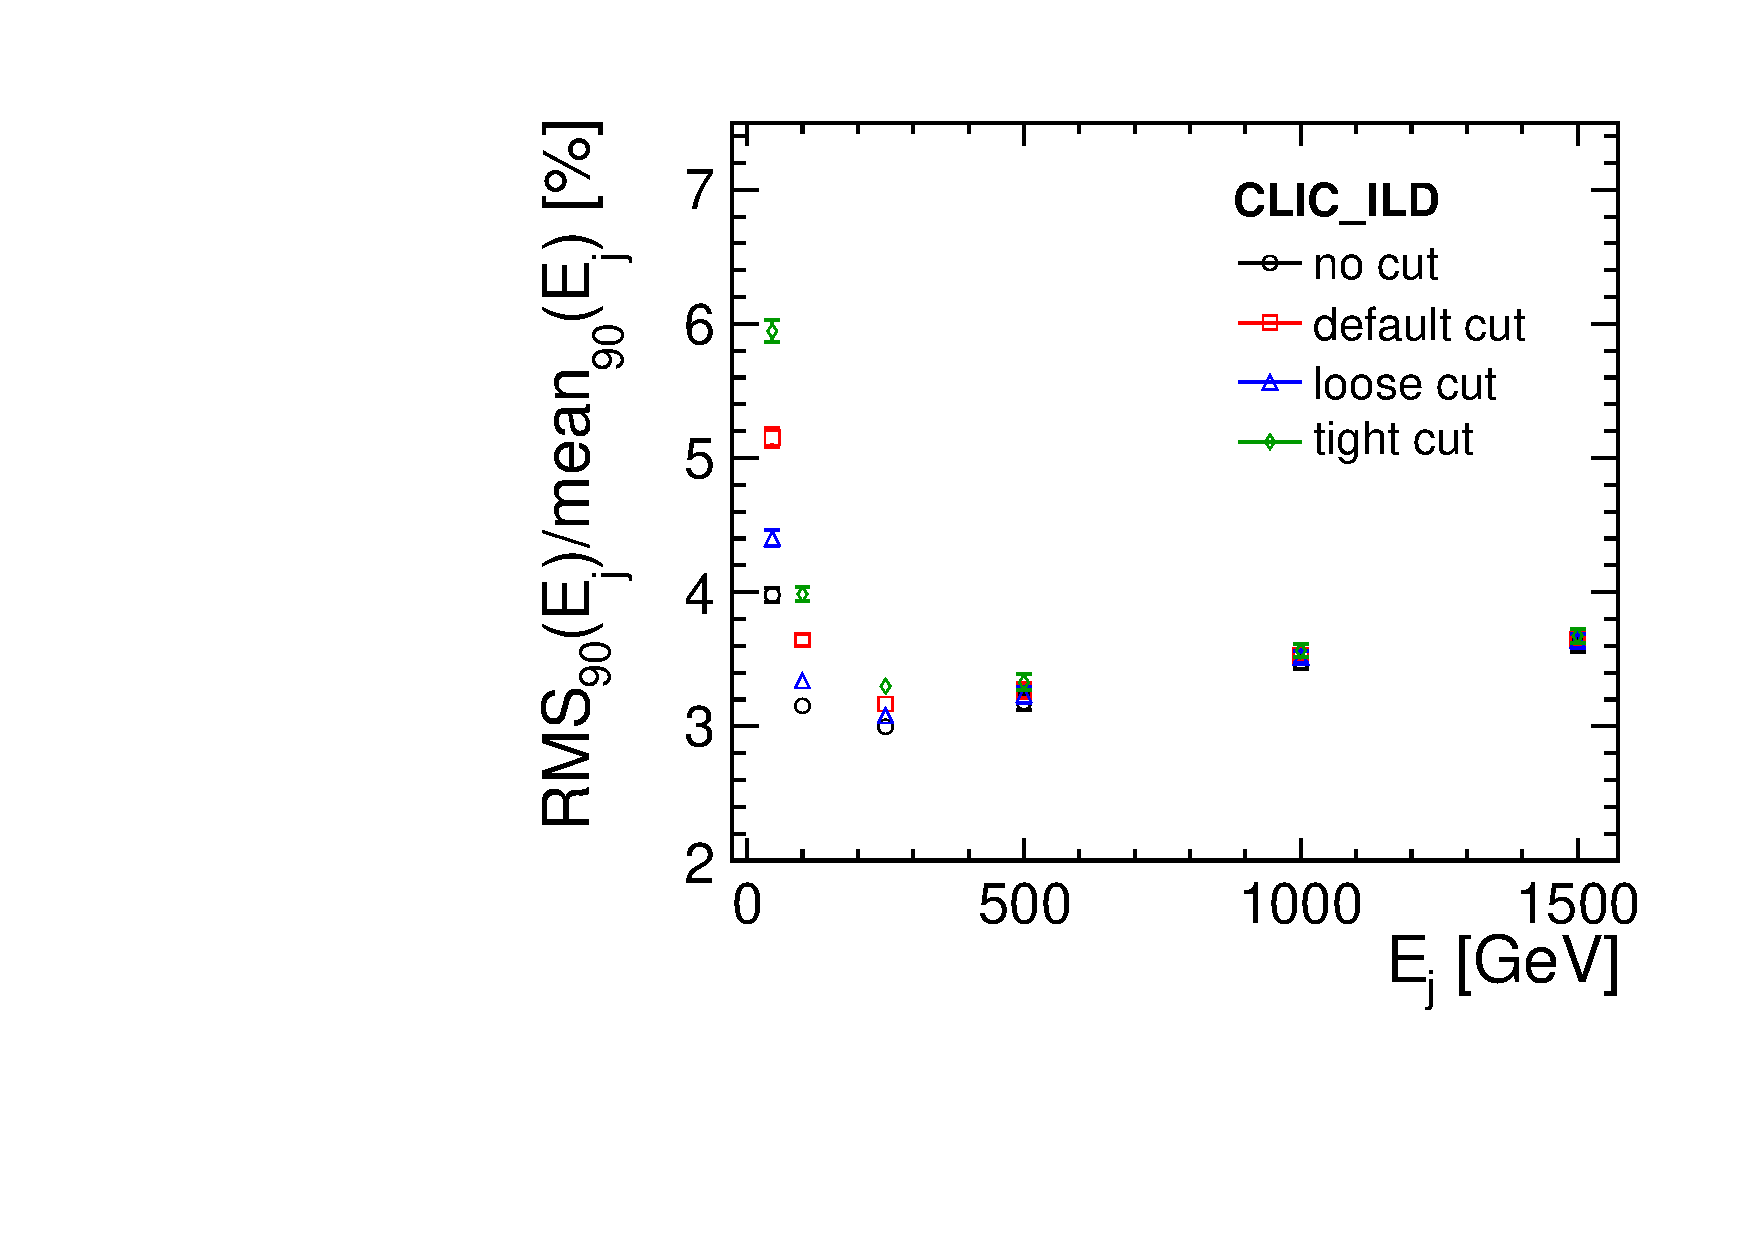
\includegraphics[width=\textwidth]{examplePlot}
    \caption{An example resolution plot from the CDR PFA performance studies.}
    \label{fig:example_res}
  \end{minipage}%
  \hfill % fill the space between the figures
  \begin{minipage}[b]{0.48\textwidth}
    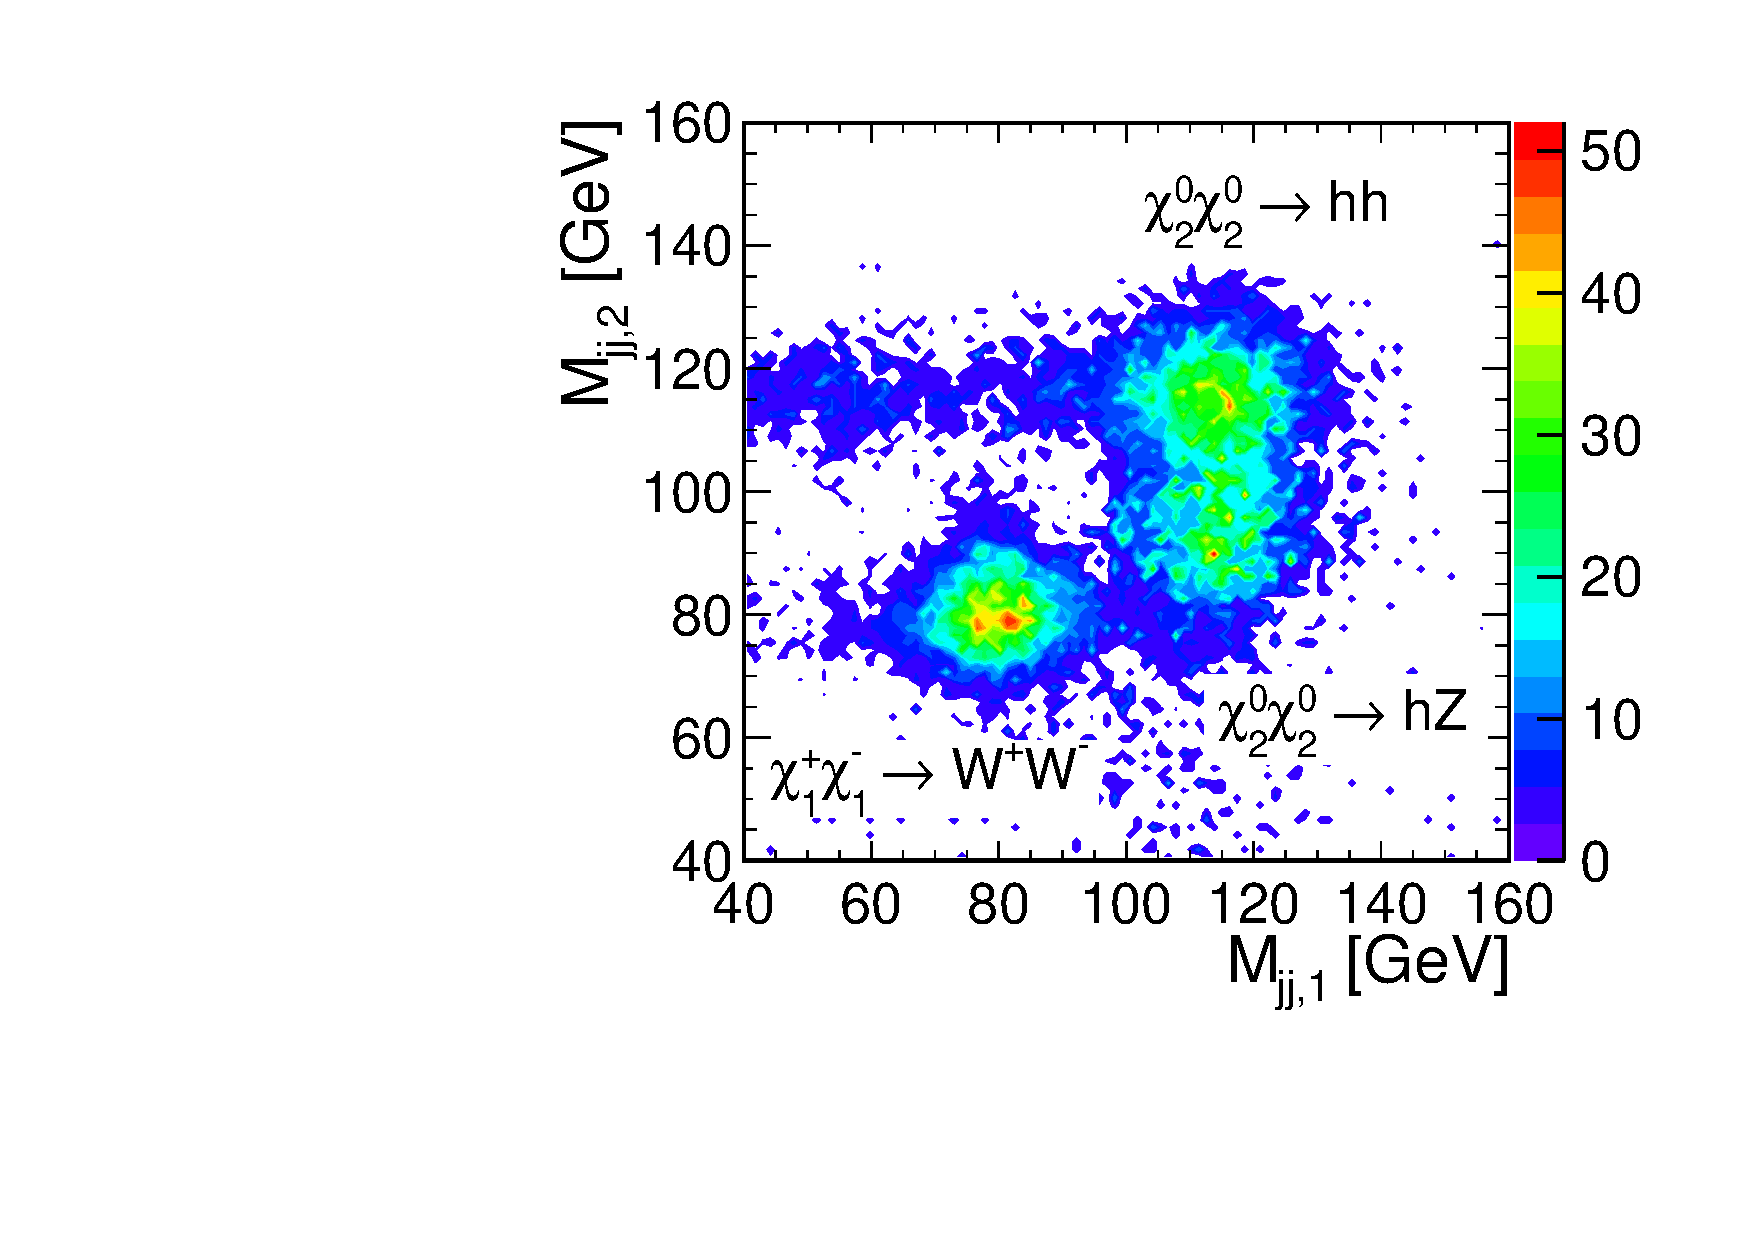
\includegraphics[width=\textwidth]{examplePlot2D}
    \caption{A 2D example plot from the CDR chargino analysis.}
    \label{fig:example_2D}
  \end{minipage}
\end{figure}

\begin{lstlisting}[language=TeX]
\begin{figure}
  \begin{minipage}[b]{0.48\textwidth}
    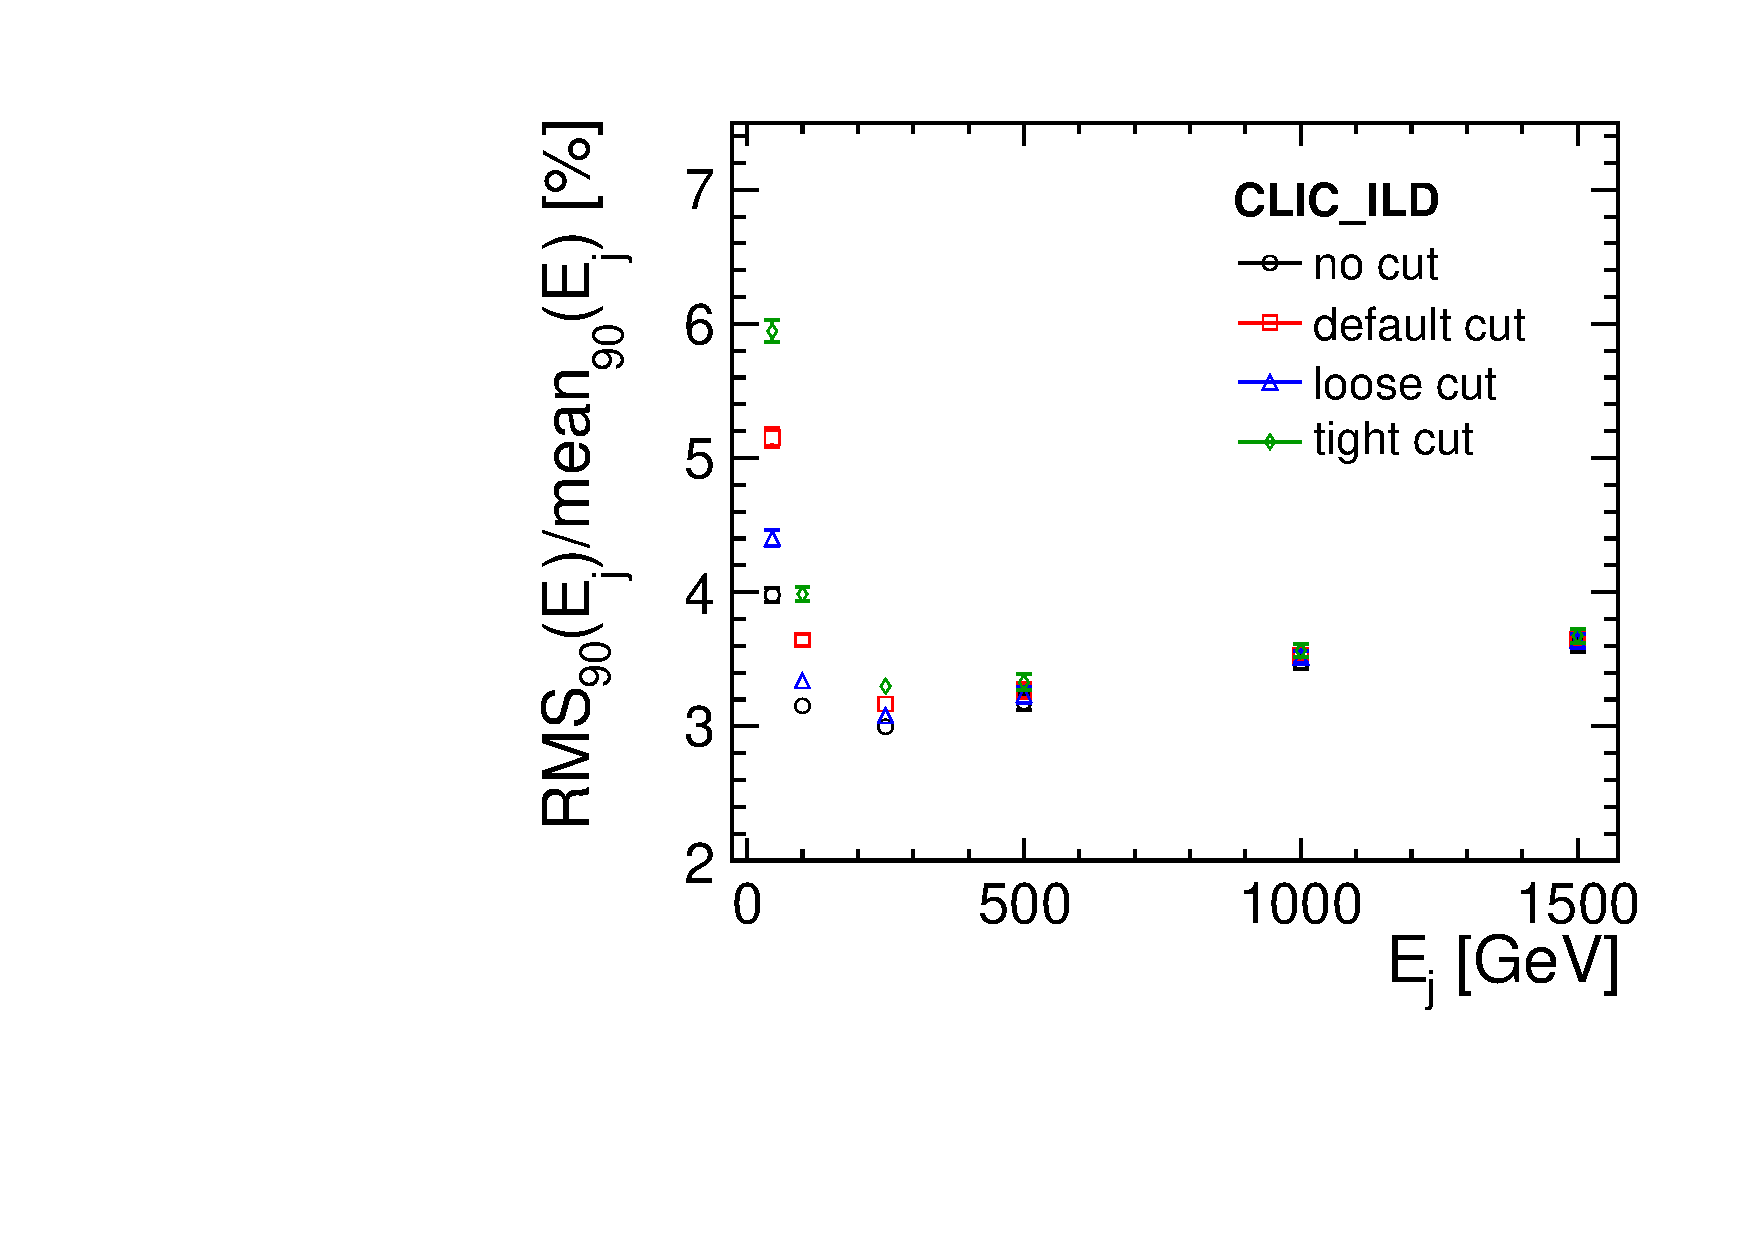
\includegraphics[width=\textwidth]{examplePlot}
    \caption{An example resolution plot from the CDR PFA performance studies.}
    \label{fig:example_res}
  \end{minipage}%
  \hfill % fill the space between the figures
  \begin{minipage}[b]{0.48\textwidth}
    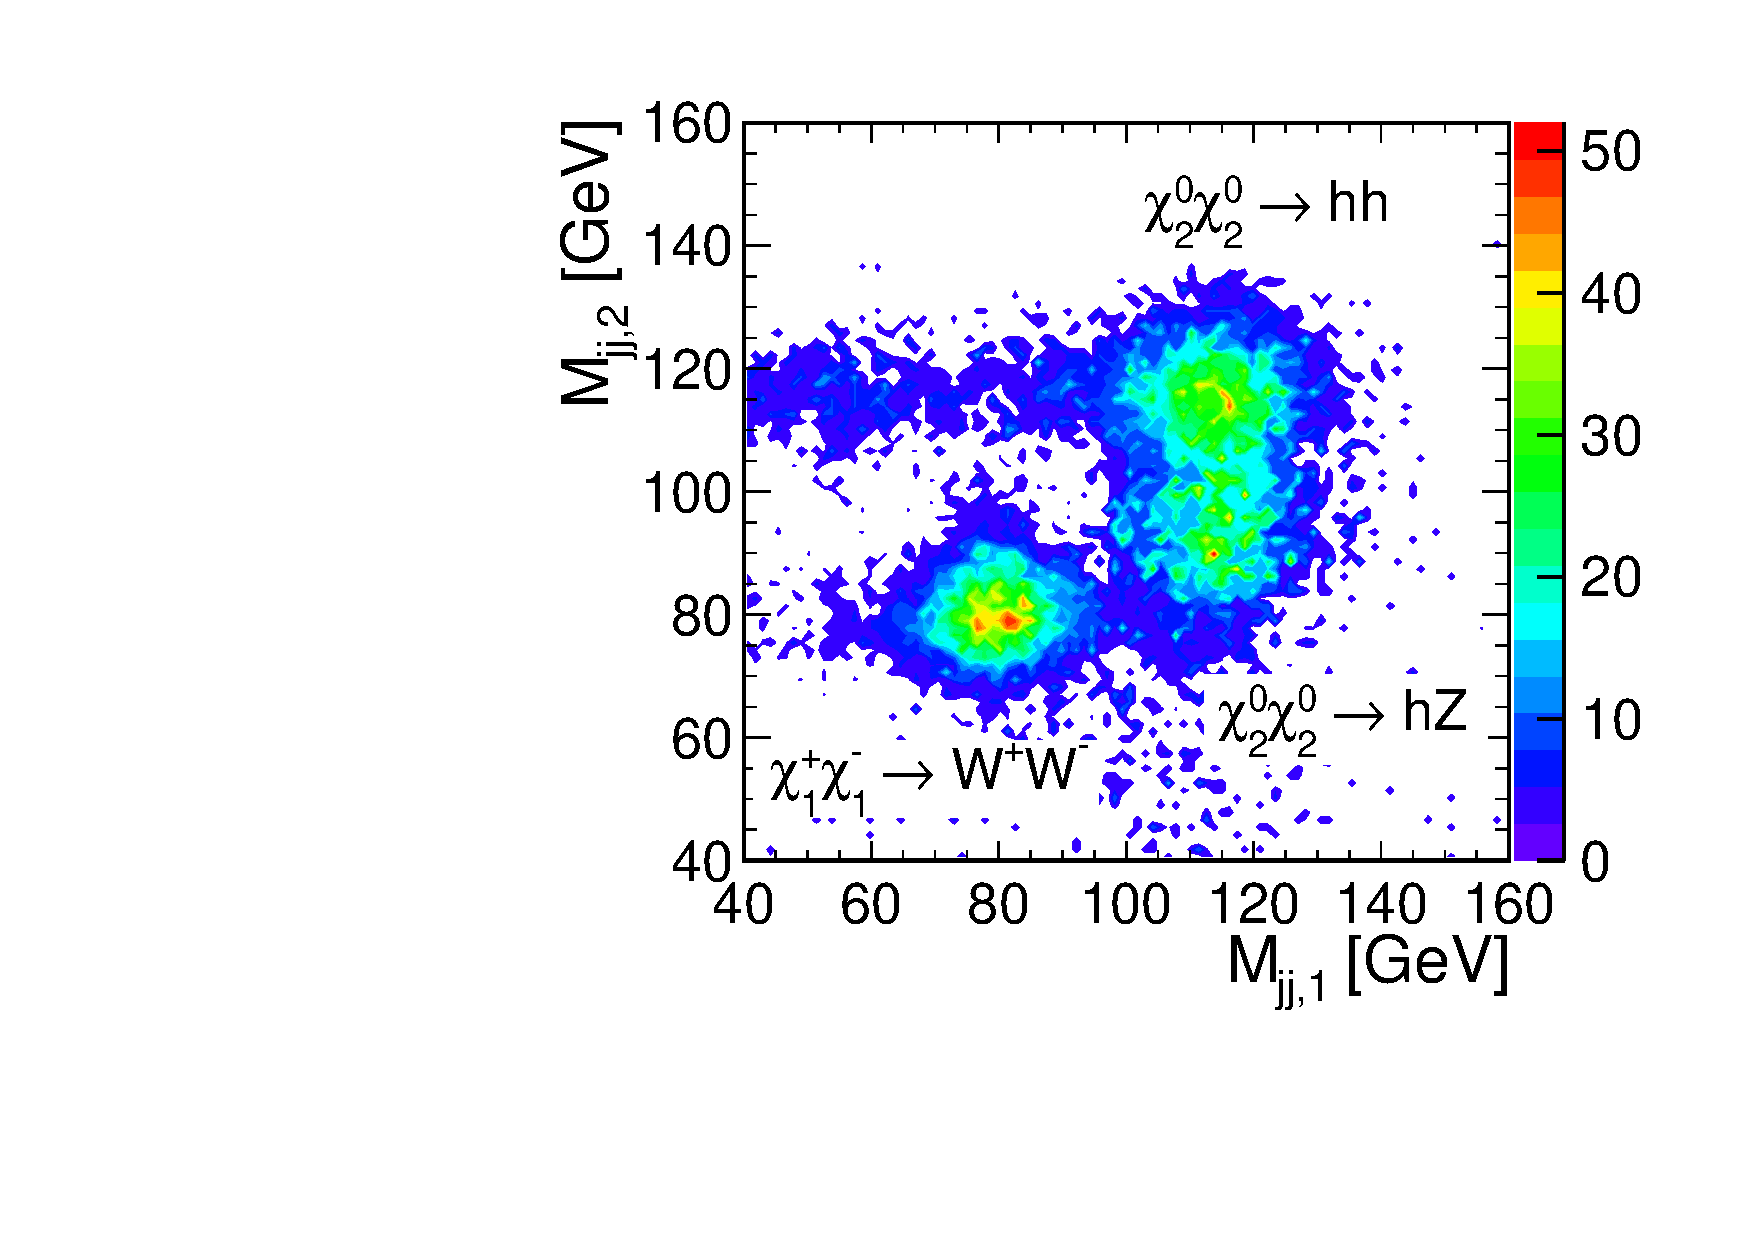
\includegraphics[width=\textwidth]{examplePlot2D}
    \caption{A 2D example plot from the CDR chargino analysis.}
    \label{fig:example_2D}
  \end{minipage}
\end{figure}
\end{lstlisting}
If the two figures are directly related, a setup with one common caption and (optionally) two sub captions might be preferred, as shown in \cref{fig:example_analysis}. This layout can be achieved using the \texttt{subcaption} package. It also allows to refer to the subfigures directly by referring to their caption: \cref{fig:example_fit,fig:example_stacked}.

\begin{lstlisting}[language=TeX]
\begin{figure}
  \centering
  \begin{subfigure}[b]{0.48\textwidth}
    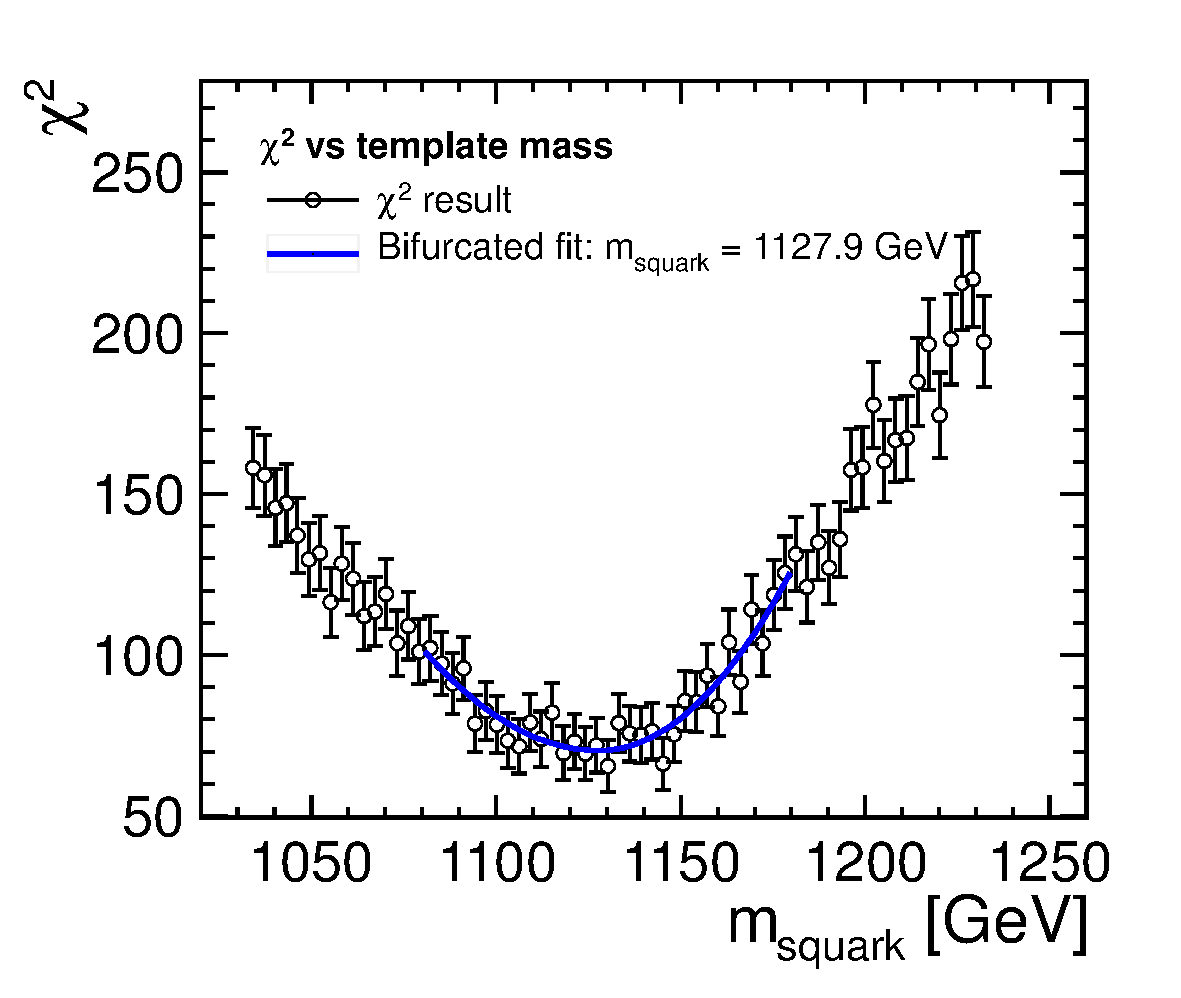
\includegraphics[width=\textwidth]{examplePlotFit}
    \caption{Template fit result}
    \label{fig:example_fit}
  \end{subfigure}
  \hfill
  \begin{subfigure}[b]{0.48\textwidth}
    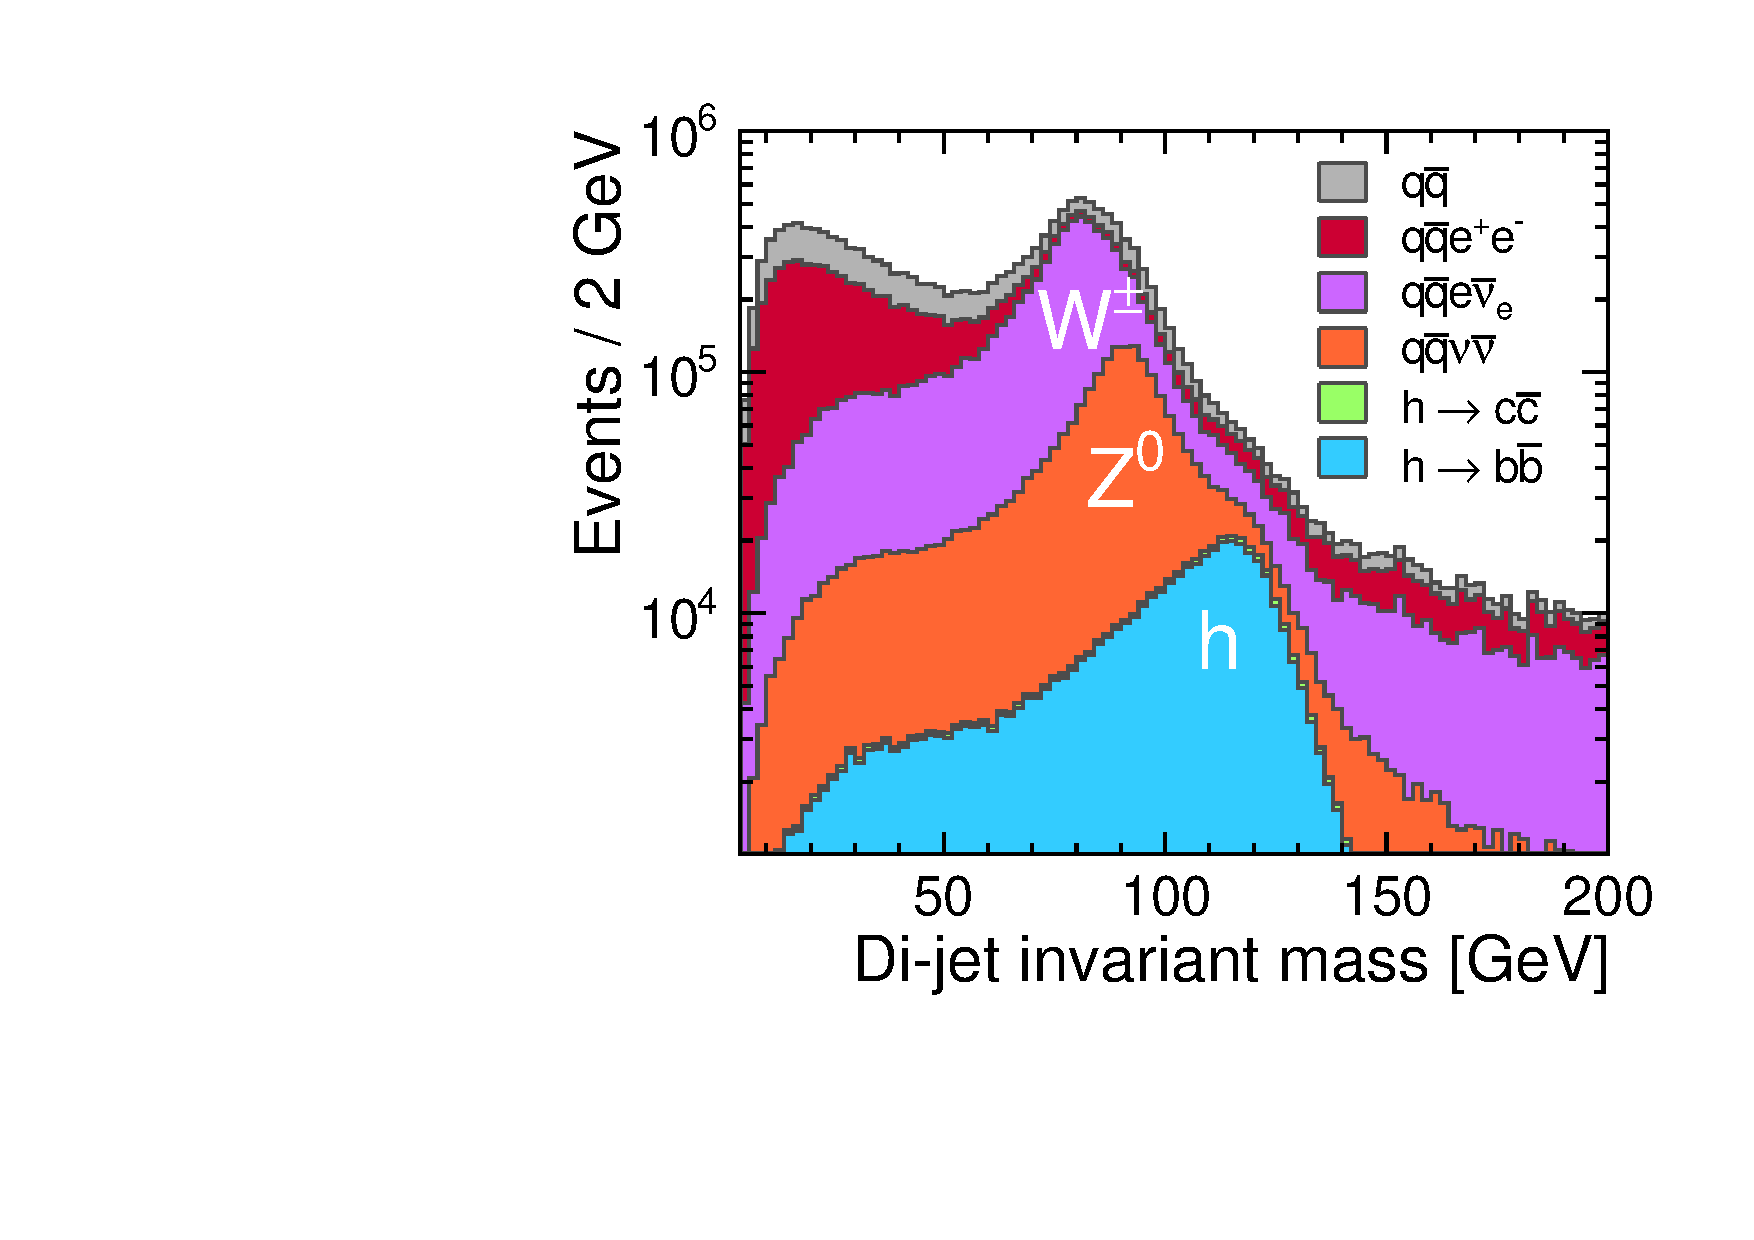
\includegraphics[width=\textwidth]{examplePlotStacked}
    \caption{Stacked histogram}
  \label{fig:example_stacked}
  \end{subfigure}
  \caption{Two example of plots from the CDR physics analysis. \subref{fig:example_fit} a template fit from the squark analysis and \subref{fig:example_stacked} a stacked histogram from the $\PH \to \PQb\PAQb$ analysis.}\label{fig:example_analysis}
\end{figure}
\end{lstlisting}

\begin{figure}
  \centering
  \begin{subfigure}[b]{0.48\textwidth}
    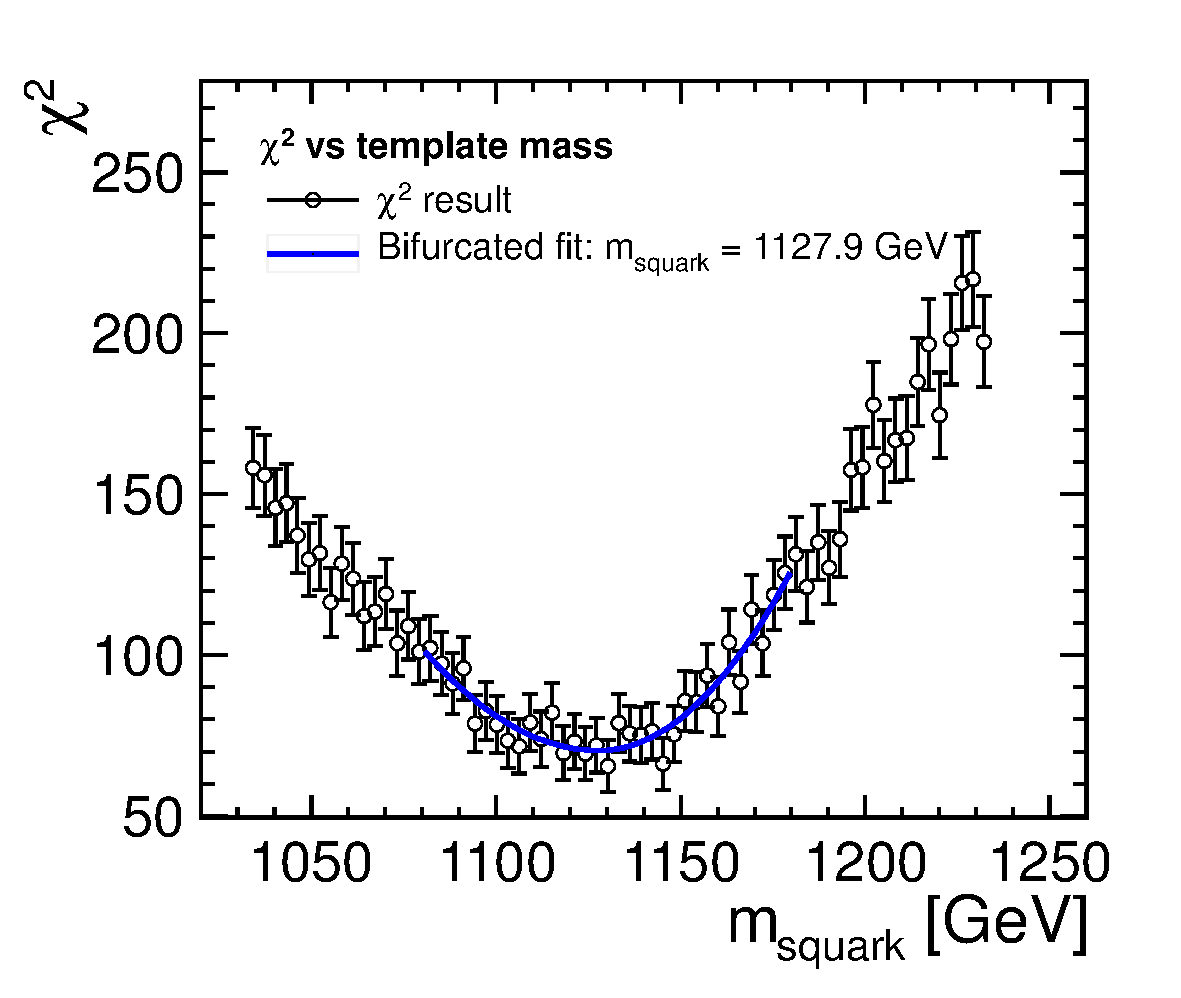
\includegraphics[width=\textwidth]{examplePlotFit}
    \caption{Template fit result}
    \label{fig:example_fit}
  \end{subfigure}
  \hfill
  \begin{subfigure}[b]{0.48\textwidth}
    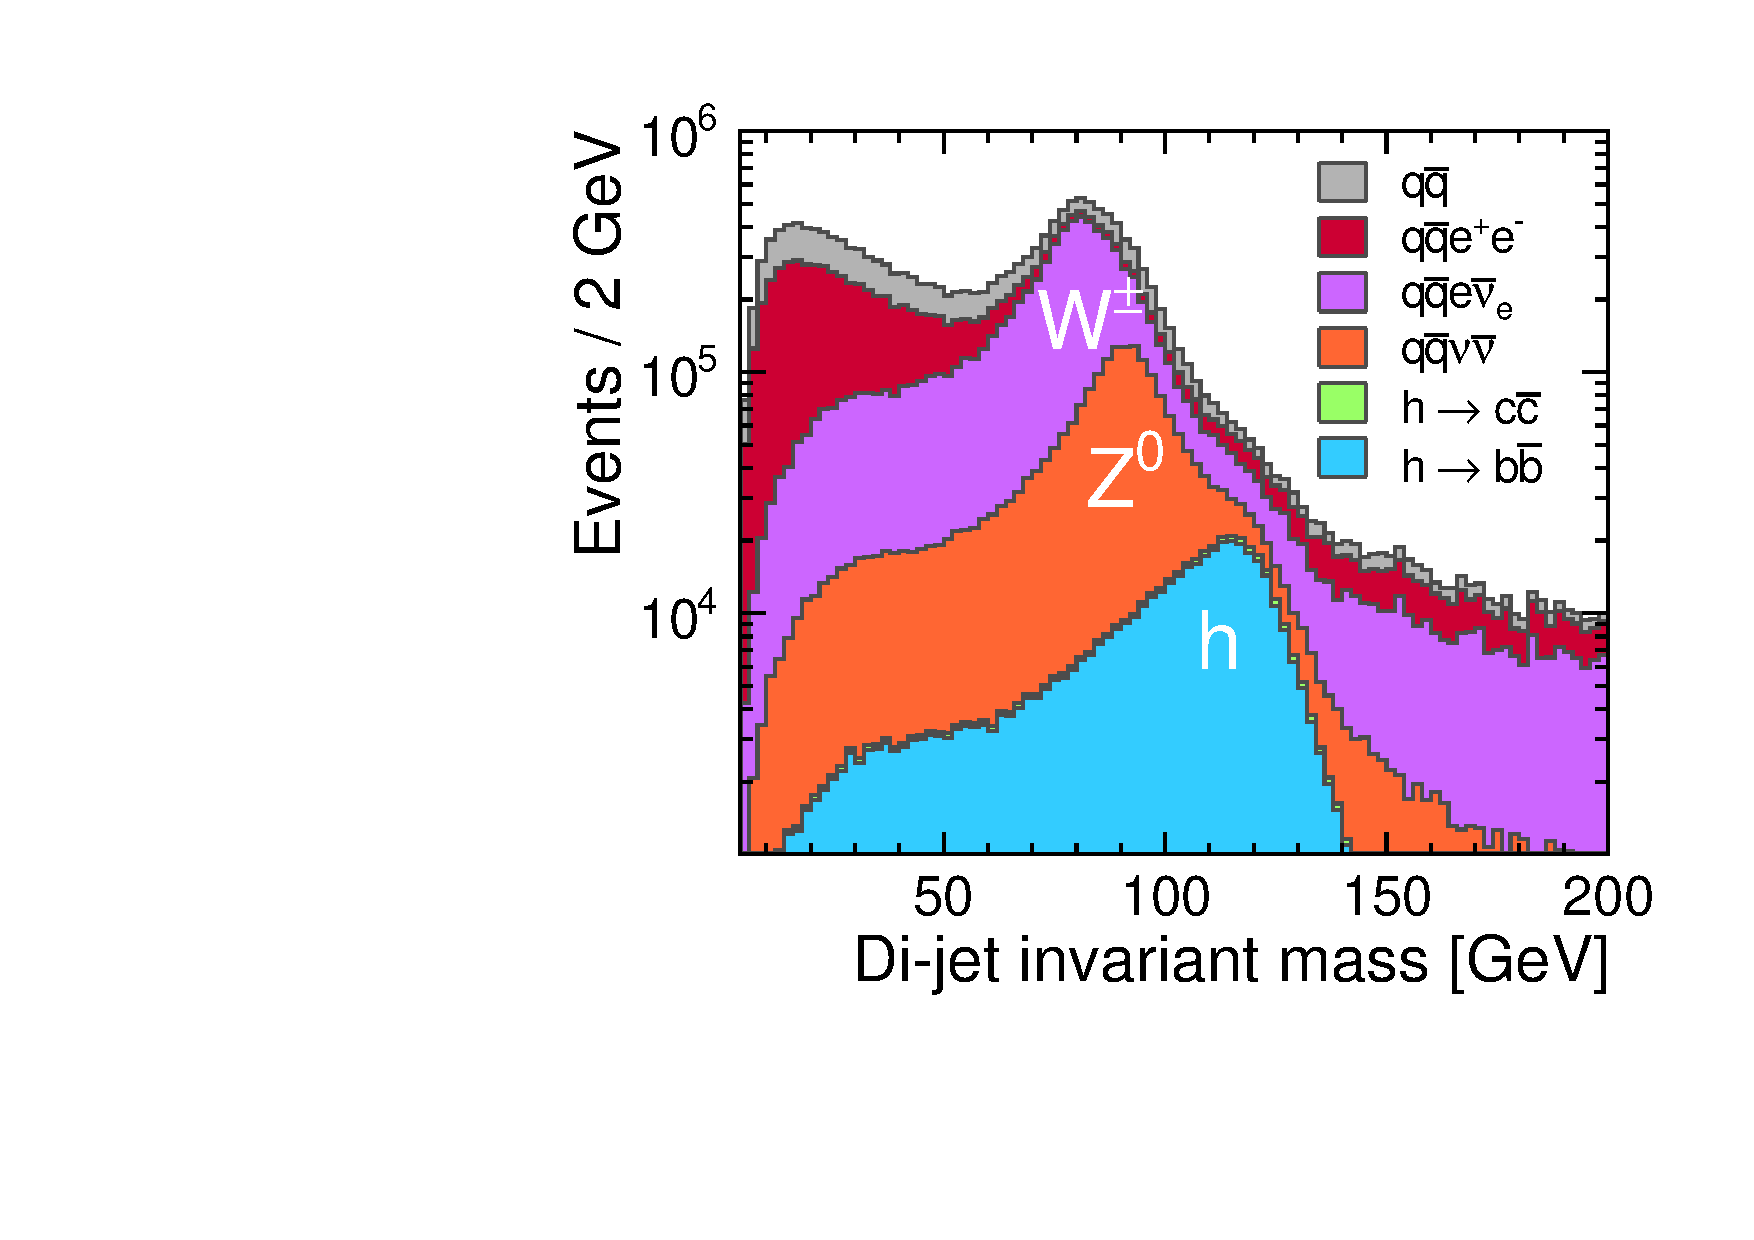
\includegraphics[width=\textwidth]{examplePlotStacked}
    \caption{Stacked histogram}
  \label{fig:example_stacked}
  \end{subfigure}
  \caption{Two example of plots from the CDR physics analysis. \subref{fig:example_fit} a template fit from the squark analysis and \subref{fig:example_stacked} a stacked histogram from the $\PH \to \PQb\PAQb$ analysis.}\label{fig:example_analysis}
\end{figure}
Tables are typically placed centered with their caption above. Unnecessary lines should be avoided to improve readability. Vertical lines are usually not required.
The horizontal lines in tables should be typeset using the commands from the \texttt{booktabs} package: \texttt{\textbackslash toprule}, \texttt{\textbackslash midrule} and \texttt{\textbackslash bottomrule}. An example table is shown in \cref{tab:machine_parameters}, which also illustrates the use of the \texttt{\textbackslash multicolumn} command.

\begin{table}
\centering
\caption{This is an example table showing the machine parameters for CLIC and the ILC for different centre-of-mass energy stages. It also demonstrates the typesetting of numbers and units using the \texttt{siunitsx} package (see \cref{sec:units}) together with the column option \texttt{S}, resulting in centered decimal points.}
\label{tab:machine_parameters}
\begin{tabular}{c S S S S}
\toprule
  & \multicolumn{2}{c}{ILC (TDR)} & \multicolumn{2}{c}{CLIC (CDR)} \\
\cmidrule(r){2-5}
 Parameter  & \SI{500}{\GeV} & \SI{1}{\TeV} & \SI{500}{\GeV} & \SI{3}{TeV} \\
\midrule
 $\theta_c\ [\si{\mrad}]$ & 14 & 14 & 20 & 20 \\
 $f_\text{train}\ [\si{\Hz}]$ & 5 & 4 & 50 & 50 \\
 $n_\text{bunches}$ & 1312 & 2450 & 354 & 312 \\
 $\Delta t\ [\si{\ns}]$ & 554 & 366 & 0.5 & 0.5 \\
 $N\ [\num{e9}]$ & 20.0 & 17.4 & 6.9 & 3.72 \\
 $\sigma_x\ [\si{\nm}]$ & 474 & 481 & 202 & 45 \\
 $\sigma_y\ [\si{\nm}]$ & 5.9 & 2.8& 2.3 & 1 \\
 $\sigma_z\ [\si{\micron}]$ & 300 & 250 & 72 & 44 \\
 $\lumi\ [\SI{e34}{\per\square\cm\per\s}]$ & 1.8 & 3.6 & 2.3 & 5.9 \\
 $\lumi_{\SI{1}{\percent}}\ [\SI{e34}{\per\square\cm\per\s}]$ & 1.0 & 2.1 & 1.4 & 2.0 \\
 $\Delta E/ E$ & 0.045 & 0.056 & 0.07 & 0.28 \\
 $N_\text{coh}$ &  &  & 200 & \num{6.8e8}\\
 $E_\text{coh}\ [\si{\TeV}]$ &  &  & 15 & \num{2.1e8} \\
 $N_\text{incoh}$ & \num{1.4e5} & \num{2.0e5} & \num{8.0e4} & \num{3.0e5}\\
 $E_\text{incoh}\ [\si{\TeV}]$ & 344 & \num{1.3e3} & \num{3.6e3} & \num{2.3e4} \\
 $n_\text{had}$ & 1.2 & 2.7 & 0.3 & 3.2 \\
\bottomrule
\end{tabular}
\end{table}

Cross references should be typed in capital letters, \ie figures should be referred to as Figure~1, sections as Section~1, \etc This behavior is easily achieved by using the commands provided by the \texttt{cleverref} package. It automatically determines the type of the reference and prepends it to the number, \ie simply type \texttt{\textbackslash cref\{LABEL\}} instead of \texttt{Figure\textasciitilde\textbackslash ref\{LABEL\}} in case of figures. The package also treats lists of labels correctly, \eg simply type \texttt{\textbackslash cref\{LABEL1, LABEL2, \dots\}} in order to refer to multiple items. Using the \texttt{\textbackslash Cref\{LABEL\}} command enforces capitalization which should be used at the beginning of a sentence, in case the configuration is changed from upper case to lower case labels.

All tables and figures that are included should be referenced in the text. Ideally the figure or table should appear on the page of the first reference to it or the following page.


\section{Particle names}
\label{sec:particles}

Particles should be typeset in normal font instead of italics, following the Particle Entity Notation scheme (PEN). Macros for all particles in high energy physics following this scheme are provided by the \texttt{heppennames2} package, which is included in this template. The following are some examples for the most common particles:
\begin{itemize}
  \item Leptons: \Pl, \PAl, \Pe, \PGm, \PGt, \Pepm, \PGmp, \PGtm, \PGn, \PAGn, \PGne, \PAGnGm
  \lstset{language=TeX}
  \begin{lstlisting}
\Pl, \PAl, \Pe, \PGm, \PGt, \Pepm, \PGmp, \PGtm, \PGn, \PAGn, \PGne, \PAGnGm
  \end{lstlisting}
  \item Quarks: \PQq, \PQu, \PQd, \PQs, \PQc, \PQb, \PQt, \PAQq, \PAQu, \PAQd, \PAQs, \PAQc, \PAQb, \PAQt
  \begin{lstlisting}
\PQq, \PQu, \PQd, \PQs, \PQc, \PQb, \PQt, \PAQq, \PAQu, \PAQd, \PAQs, \PAQc, \PAQb, \PAQt
  \end{lstlisting}
  \item Gauge bosons and scalar bosons: \PGg, \PW, \PWpm, \PWp, \PWm, \PZ, \Pg, \PH
  \begin{lstlisting}
\PGg, \PW, \PWpm, \PWp, \PWm, \PZ, \Pg, \PH
  \end{lstlisting}
  \item Mesons: \PGp, \PGpz, \PGppm, \PKmp, \PKzL, \PKzS
  \begin{lstlisting}
\PGp, \PGpz, \PGppm, \PKmp, \PKzL, \PKzS
  \end{lstlisting}
  \item Beyond the Standard Model: \PZpr, \PSh, \PSA, \PSHpm, \PSg, \PSGczDo, \PSGcpDt, \PSQ, \PASQ, \PSeL, \PSGmmR, \PXXG, \PXXSG
  \begin{lstlisting}
\PZpr, \PSh, \PSA, \PSHpm, \PSg, \PSGczDo, \PSGcpDt, \PSQ, \PASQ, \PSeL, \PSGmmR, \PXXG, \PXXSG
  \end{lstlisting} 
\end{itemize}


\section{Units}
\label{sec:units}

Units should always be typeset in normal font and not in italics. A number and its unit should be separated by a thin space, \eg 10\,\text{GeV} instead of 10 GeV or 10GeV. This can be achieved by typing \texttt{10\textbackslash,\textbackslash text\{GeV\}.} The \texttt{\textbackslash text} keyword ensures normal font also in math environments. Degrees and percent should have no space if preceded by a number, \ie 22\degrees and 50\%.

All of this can be easily achieved by using the \texttt{siunitx} package which is already configured in this template. It provides macros for most units used in physics, and automatically treats ranges of numbers as well as uncertainties. Simple numbers can be written by \texttt{\textbackslash num\{NUMBER\}}, units without numbers are written as \texttt{\textbackslash si\{UNIT\}} and numbers with units can be written as \texttt{\textbackslash SI\{NUMBER\}\{UNIT\}}. The following are a few examples:
\begin{itemize}
  \item \texttt{\textbackslash num\{1.3e4\}} results in \num{1.3e4}
  \item \texttt{\textbackslash SI\{15\}\{\textbackslash kg\textbackslash m\textbackslash per\textbackslash s\}} results in \SI{15}{\kg\m\per\s}.
  \item \texttt{\textbackslash SI\{2+-0.01\}\{\textbackslash per\textbackslash ab\}} results in \SI{2.0+-0.01}{\per\ab}.
  \item \texttt{\textbackslash SIlist\{10;20;30\}\{\textbackslash MeV\}} results in \SIlist{10;20;30}{\MeV}.
  \item \texttt{\textbackslash SIrange\{1\}\{100\}\{\textbackslash GHz\}} results in \SIrange{1}{100}{\GHz}.
  \item \texttt{\textbackslash SI\{50\}\{\textbackslash percent\}} results in \SI{50}{\percent}.
  \item \texttt{\textbackslash SI\{22\}\{\textbackslash degree\}} results in \SI{22}{\degree}. (Alternatively use \texttt{\textbackslash ang\{22\}} for the same result: \ang{22}).
\end{itemize}


\section{References and citations}
\label{sec:cite}
Citations should be indicated by a number in square brackets. Use a tilde between the text and the cite command to create a whitespace that is not broken over two lines, \ie \texttt{text\textasciitilde\textbackslash cite\{REFERENCE\}}. The references should be listed in the order they appear in the document. This is done automatically by \latex, but otherwise must be done by the author.

The style adopted for the references is that titles of articles or books are given in italics, volumes of journals are given in bold font and everything else is given in normal font. The citations should look as follows:
\begin{itemize}
  \item Journal articles: Author(s), \textit{Title}, Journal \textbf{Volume} (Year) First page, DOI, arXiv number.
  \item Books: Author(s), \textit{Title}, Edition, Publisher, Location, Year.
  \item Notes: Author(s), \textit{Title}, Note number, Institute, Year, DOI, arXiv number.
\end{itemize}
In case of more than three authors only the first author should be given followed by ``et al.''. In case of editor(s) the names should be followed by ``, ed(s).''. Only the first page is given in case of page ranges and no pagination, \ie ``p.'' or ``pp.'', is added in case of journals. The DOI and arXiv numbers should be added as hyperlinks if available. For references that are not published in a journal (\eg the AIDAinnova note series), the note number can be made a hyperlink to the document location, \ie the record on the CERN Document Server (CDS).

The \latex template has the styling defined in the \path{AIDAinnova_biblatex.sty} and no additional configuration is required beyond providing all necessary fields in the \path{.bib} file(s) for the references. As examples we cite some journal articles~\cite{Higgs:1964pj,Aad:2012tfa,Chatrchyan:2012ufa}, some books~\cite{Griffiths:111880,Gunion:322177}, a report with editors~\cite{cdrvol2}, a note~\cite{Redford:1690648}, proceedings~\cite{Schulte:2001aw} and a url~\cite{lcio}. The resulting style can be seen in the references below.

\section{Licence}
\label{sec:licence}
All documents (except for drafts) are by default covered by the open access license CC-BY-4.0. Although the majority of the journals of interest for the high-energy physics community today publish under open access there are still some exceptions. It is the responsibility of the author to inform the publications committee about the intended submission to a non open access journal. The committee will then take the appropriate steps to ensure that the publication is treated according to the rules. Please contact the publications committee for any questions regarding your particular document. The licence statement can be removed from the cover page by uncommenting the line \texttt{\textbackslash nolicence} in your document. Note that the licence statement is never shown for documents while in draft mode. Read more about the licence here: \href{https://creativecommons.org/licenses/by/4.0/}{https://creativecommons.org/licenses/by/4.0/}.





% add references
\printbibliography[title=References]

\end{document}
